\documentclass[aspectratio=169,12pt]{ctexbeamer}
\usetheme{default}
\useinnertheme{SimplePlus}
\usecolortheme{SimplePlus}
\usepackage{chemformula} %化学公式宏包
\usepackage[version=4]{mhchem} %化学公式宏包
\usepackage{siunitx} %数字，单位宏包
    \sisetup{
	separate-uncertainty = true,
	inter-unit-product = \ensuremath{{}\cdot{}}
    } %单位间加小圆点
\usepackage[all]{xy}  %XY-pic 交换图包
\usepackage{booktabs} %三线表
\usepackage{multirow} %合并单元格
\usepackage{makecell} %表格内强制换行
\usepackage{colortbl} %彩色表格需要加载的宏包
\usepackage{xcolor}
%修改公式间距
\makeatletter
\renewcommand\normalsize{%
\abovedisplayskip 6\p@ \@plus2\p@ \@minus5\p@
\abovedisplayshortskip \z@ \@plus3\p@
\belowdisplayshortskip 6\p@ \@plus3\p@ \@minus3\p@
\belowdisplayskip \abovedisplayskip
\let\@listi\@listI}
\makeatother


%微分符号
\makeatletter
\newcommand*{\dif}{\mathop{}\!\mathrm{d}}
\makeatother

%自定义颜色
\newcommand*{\cred}{\textcolor{red}}
\newcommand*{\cblue}{\textcolor{blue}}
\newcommand*{\cgreen}{\textcolor{green}}
\newcommand*{\ccyan}{\textcolor{cyan}}
\newcommand*{\cmagenta}{\textcolor{magenta}}
\newcommand*{\cyellow}{\textcolor{yellow}}
\definecolor{DarkBlue}{RGB}{1,126,218}
\newcommand*{\cdarkblue}{\textcolor{DarkBlue}}

%\setbeamertemplate{background}{\includegraphics[height=\paperheight]{bg.pdf}}
\setbeamertemplate{navigation symbols}{}   %取消导航条
\setbeamertemplate{footline}[frame number]    %页码
\setbeamerfont{frametitle}{size=\fontsize{16}{20}}  %标题
\setbeamerfont{framesubtitle}{size=\fontsize{10}{12}}  %副标题
%item列表符号使用小圆点
\setbeamertemplate{itemize item}{$\bullet$}

\linespread{1.2}

%突出本章标题
\AtBeginSection[]
{
	\begin{frame}{目录}
		\transfade%淡入淡出效果
		\tableofcontents[sectionstyle=show/shaded] %突出显示当前章节，其它章节淡化
		\addtocounter{framenumber}{-1}  %目录页不计算页码
	\end{frame}
}

%字体
\usefonttheme{serif}
\setmainfont{Times New Roman}
\usepackage{amsmath}
\usepackage{unicode-math}
\setmathfont{XITS Math}

%直立积分
\DeclareSymbolFont{EulerExtension}{U}{euex}{m}{n}
\DeclareMathSymbol{\euintop}{\mathop} {EulerExtension}{"52}
\DeclareMathSymbol{\euointop}{\mathop} {EulerExtension}{"48}
\let\intop\euintop
\let\ointop\euointop

%封面
\title{\Huge 化工设计}
\subtitle{\large 反应器，物料衡算，能量衡算}
\author{张斌}
\institute[河北农业大学 理工系]{\normalsize 河北农业大学 理工系}
\date{}



\begin{document}

	%封面
\begin{frame}
		\titlepage
		\thispagestyle{empty}
		\addtocounter{framenumber}{-1}
\end{frame}

\begin{frame}
        \frametitle{釜式反应器}
			\bigskip
        	\begin{minipage}{0.48\linewidth}
				\begin{figure}[htpb]
					\centering
					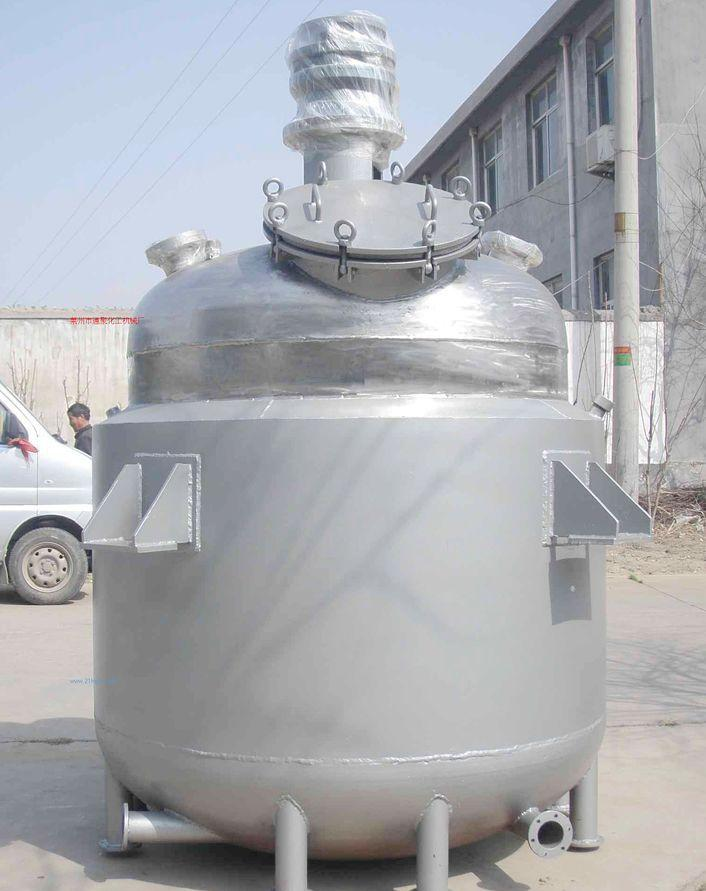
\includegraphics[width=.8\linewidth]{figures/fushi.jpg}
				\end{figure}
			\end{minipage}\hfill
			\begin{minipage}{0.48\linewidth}
				\begin{figure}[htpb]
					\centering
					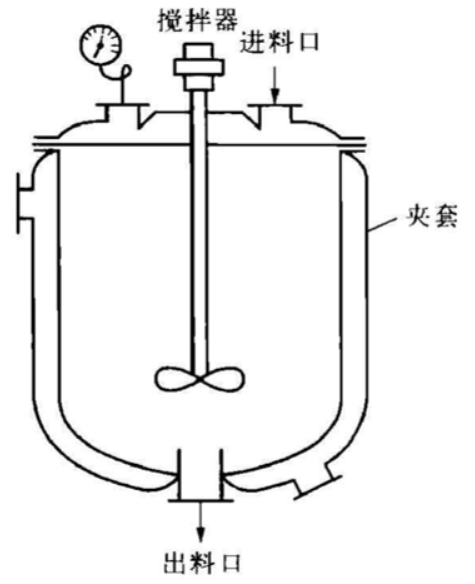
\includegraphics[width=.8\linewidth]{figures/fushi2.png}
				\end{figure}
			\end{minipage}   
\end{frame}


\begin{frame}
	\frametitle{釜式反应器\ \small{适用反应类型}}
	\begin{itemize}
		\item 均相反应
		\begin{itemize}
			\item[\bigcirc] 主要是液相均相反应
		\end{itemize}
		\item 多相反应
		\begin{itemize}
			\item[\bigcirc] 气液
			\item[\bigcirc] 液固
			\item[\bigcirc] 液液
			\item[\bigcirc] 气液固
		\end{itemize}
	\end{itemize}
\end{frame}


\begin{frame}
	\frametitle{釜式反应器\ \small{操作方式}}
	工业反应器根据其流体流动方式分为连续流动和间歇操作两种。
	\begin{enumerate}
		\item 间歇操作
		\begin{itemize}
			\item[\bigcirc] 适用于时间长的反应，如聚合物生产、生物发酵等。
			\item[\bigcirc] 产品批量小、品种不断变化的加工过程，如精细化学品生产、合成制药等。
		\end{itemize}
		\item 连续操作
		\begin{itemize}
			\item[\bigcirc] 在大规模生产过程中，多采用物料连续流动的操作方式
			\item[\bigcirc] 如石油炼制、乙烯生产、天然气转化、氨和尿素的合成等
		\end{itemize}
	\end{enumerate}
	
\end{frame}


\begin{frame}
	\frametitle{管式反应器}
	\bigskip
        	\begin{minipage}{0.48\linewidth}
				\begin{figure}[htpb]
					\centering
					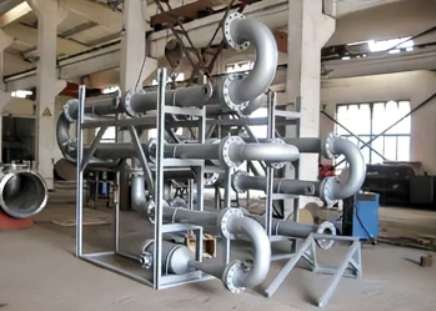
\includegraphics[width=.8\linewidth]{figures/guanshi.png}
				\end{figure}
			\end{minipage}\hfill
			\begin{minipage}{0.48\linewidth}
				\begin{itemize}
					\item 多数采用连续操作
					\item 少数采用半间歇操作
					\item 间歇操作，罕见
				\end{itemize}
			\end{minipage}  
\end{frame}





\end{document}